\section{Discussion}
In this project we propose a model mapping some spatio-temporal data into a
map once getting such dataset from Twitter. This model successfully take
pre-processed twitter data and return visualized result of distribution of
such data. With machine learning-based binary classification, the
spatio-temporal data now can have sentiment information as well, therefore it
is possible to visualize the the trend of people's opinion by regions and
time. This model has potential to be developed as an API automatically return
visualized map of distribution of sentiments on some issues. This may
contribute the government decision maker to refer to public opinion on a
specific issue they are interested in. 

Visualization of the spatial feature flow as the temporal data progresses is
an integral part of data warehousing and data mining techniques. Spatial data
mining requires specific trend recognition in order to make successful
conclusive argument which is visualized using the visualization technique. In
this project, we have used Geo Pandas to visualize our spatial data using
designated spatial operator. In our future studies, we would like to make the
model propose the trends in spatial data flow in maps which can be visualized
using the similar libraries.\\

\begin{figure}[H]
\centering
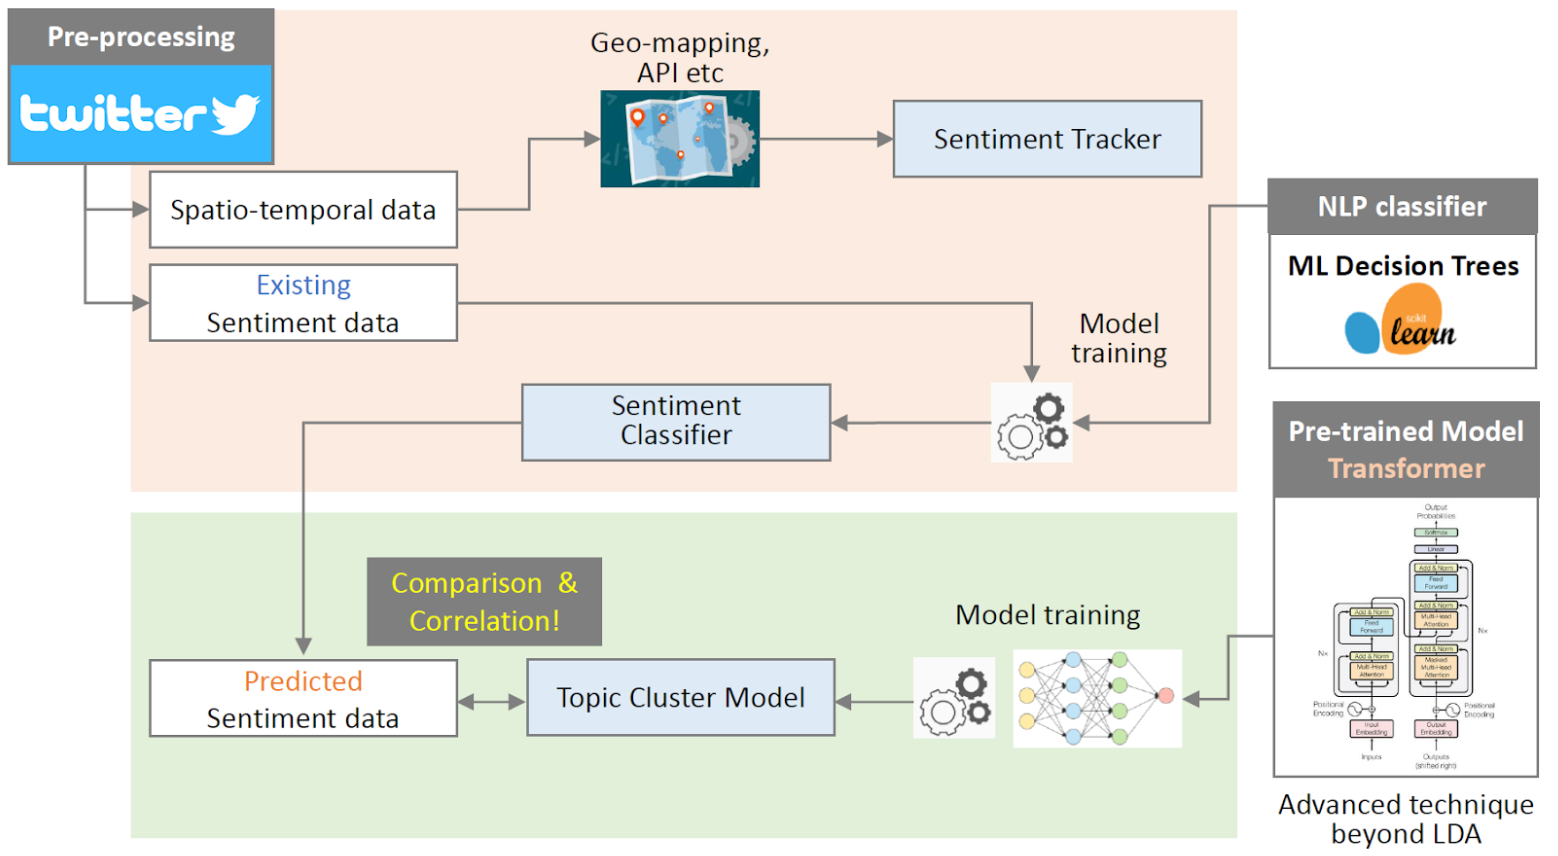
\includegraphics[width=0.5\textwidth]{imgs/Research_Process.png}
\caption{\label{fig:Research process}Future plan}
\end{figure}

However it still has a long way to go in that it is too simple for disclosing
some deeply meaningful implications. At present, since our model just
provides the spatio-temporal view of the public opinion about an issue, it
lacks further analysis about what specific topics are to be drawn from this.
To dig into this issue, we will do detailed topic clustering task to classify
how many different sub topics can be drawn from the overall topic of Covid-19
outbreak. Our topic for twitter dataset are filtered by the topic pandemic.
However this is too simple. Therefore in the longer run, we should proceed to
sub-topic clustering to get detailed areas under the single main topic. For
example, they might be either government's specific policy about the pandemic
or public opinion about some vaccine company's business guideline, and etc.

In this project, we have chosen a static method for topic clustering which is
Latent Dirichlet Allocation (LDA). Although this is static and an old method
compared to the modern deep learning approaches, our result shows its
relevancy in this domain is still present. The current research that are
going on, a lot of the authors are using LDA to get a primary insight in the
dataset that they compare with their model as a baseline. In the coming days,
our research will focus on the modern approaches using deep learning to make
compact and deployable topic clustering model.

One promising candidate for the model is the Transformer. This is a greatly
applied model architecture in Natural Language Processing now, which is based
on the core technology called the \textit{attention mechanism}. Our team
belive this should be an appropriate alternative current LDA to do the
detailed topic clustering task (Fig.21). 